\chapter{Change Point Detection} 

A change point detection algorithm is concerned to identify points in time where the statistical properties of a time series have changed. This problem have a broad application in different knowledge fields, and in general, the algorithms performance are closely related with the input characteristics. Also, when the latent information of the procedures that generated a time series are abscent the target statistical properties can be considered subjective, bringing difficulties not only in the detection phase but also in the problem formalization.

In this context this chapter specifies the problem and briefly discusses several change point detection algorithms. The literature of this area is extensive, and it is common to find methods that presents a poor performance due to a variety of reasons, such as they are too specific or because the mechanisms were only analyzed through theoretical aspects. Therefore, it was chosen a set of methods that can provide a good practical and theoretical perspective, and also flexibility to insert adaptations that can better handle some input peculiarities. Futhermore, through this chapter is exposed several obstacles when dealing with real data and some adopted solutions which are not described in literature.

\section{Problem Definition}

The problem can be categorized in offline or online. In the offline version, to decide if a specific point at time $t$ is a change point the solver has available the whole time series, including past and future information on $t$. In the other hand, in the online version the information is available up to time $t$. The choice between these options are defined by the application domain, in some cases data are processed in real time and the change points should be detected as soon as possible, but in others the change points are identifyied by historical purpouses and offline algorithms can be used. 

It is intuitive that the offline case is more robust since there are more information to make a classification. In practice, to increase the statistical confidence of a decision, the online definition is relaxed and to decide if a point at time $t$ is a change point it is possible to use data up to a small window in future of $t$, which in real time processing means that the application should wait until more data are available. This trick plays a trade-off between minimizing the time to detect a change and correctly classify a point. Therefore, in some cases, the online version can be transformed in the offline version by only modifying the input availability. 

In this work it is considered the following input and change points characteristics, which were defined considering the final application scenario:
\begin{itemize}
    \item Univariate time series. However, it is possible to easily extend several methods presented here to deal with multivariate data.
    \item Unevenly time series, that is, data is not regularly sampled in time.
    \item Unknow number of change points.
    \item Time series with different lengths.
    \item Different number of points between change points.
    \item Focus on changes in the underlying mean and distribution, disconsidering other kinds of changes such as in periodicity.
    \item Outliers are not considered statistical changes.
    \item There is no latent information of the time series.
    \item It is considered the online and offline options.
\end{itemize}

\section{Notation}

An univariate time series composed of $n$ points is defined by two vectors, $\mathbf{x} = (x_{1}, ..., x_{n})$ and $\mathbf{y} = (y_{1}, ..., y_{n})$. The value $y_{i}$ indicates the $i-$th sampled value and $x_{i}$ indicates the associated sample time. It is assumed that the points are sorted by time, that is, $x_{i - 1} < x_{i}$ for $i = 2, ..., n$. Since unevenly time series is considered, $x_{i} - x_{i - 1}$ can be different for different $i$ values. For $s \ge t$ the following convention is adopted $\mathbf{y}_{s:t} = (y_{s}, ..., y_{t})$.

The presence of $k$ change points implies that data is splitted into $k+1$ segments, also called windows. Let $\tau_{i}$ indicate the $i-$th change point for $i=1,...,k$. Also let $\tau_{0} = 0$, $\tau_{k + 1} = n$ and $\boldsymbol \tau = (\tau_{0}, ..., \tau_{k + 1})$. Then, the $i-$th segment is defined by $\mathbf{y}_{\tau_{i - 1} + 1 : \tau_{i}}$, assuming that $\tau_{i - 1} < \tau_{i}$ for $i = 1, ..., k + 1$.

Through the previous definitions, change point detection algorithms mainly aim to find both $k$ and $\boldsymbol \tau$.

\section{Sliding Window Techniques}

Sliding window techniques use two sliding windows over the time series, and reduce the problem of detecting change points to the problem of testing whether data from the windows were generated by different distributions. One approach is to consider a distance metric between two empirical distributions as the base to infer the change points. Letting $d(\mathbf{a}, \mathbf{b})$ be the distance between two empirical distributions defined by the windows $\mathbf{a}$ and $\mathbf{b}$, and considering windows of length $m$, the Algorithm~\ref{alg:sliding_window} presents a simple sliding window method.

\begin{algorithm}
    \caption{Sliding Window}
    \label{alg:sliding_window}
	\begin{algorithmic}[1]
		\State $i \gets 1$
		\While{$i + 2 m - 1 \leq n$}
             \If{$d(\mathbf{y}_{i : i + m - 1}, \mathbf{y}_{i + m : i + 2m - 1}) > \alpha$}
                \State Report $i + m - 1$ as a change point
		        \State $i \gets i + m$
             \Else
		        \State $i \gets i + 1$
             \EndIf
        \EndWhile
	\end{algorithmic}
\end{algorithm}

In this method, when the distance between the distributions is above some threshold $\alpha$ a change point is reported. This is a commom aproach for an online application, however it is possible to increase the classification accuracy in offline cases. As an example, the top plot of figure~\ref{fig:sliding_window_toy_example} presents a simulated time series, the segment $\mathbf{y}_{1 : 1000}$ was generated sampling a $N(1, 0.2)$ distribution and $\mathbf{y}_{1001 : 2000}$ was sampled through $N(5, 0.2)$. The distribution of a window was constructed using binning the data with bins of size 0.02. The bottom plot of the same figure presents the associated Hellinger distance between two sliding windows, where the point $(i, d_{i})$ represents the distance between the windows $\mathbf{y}_{i - 100 : i - 1}$ and $\mathbf{y}_{i : i + 99}$.

\begin{figure}[H]
    \centering
    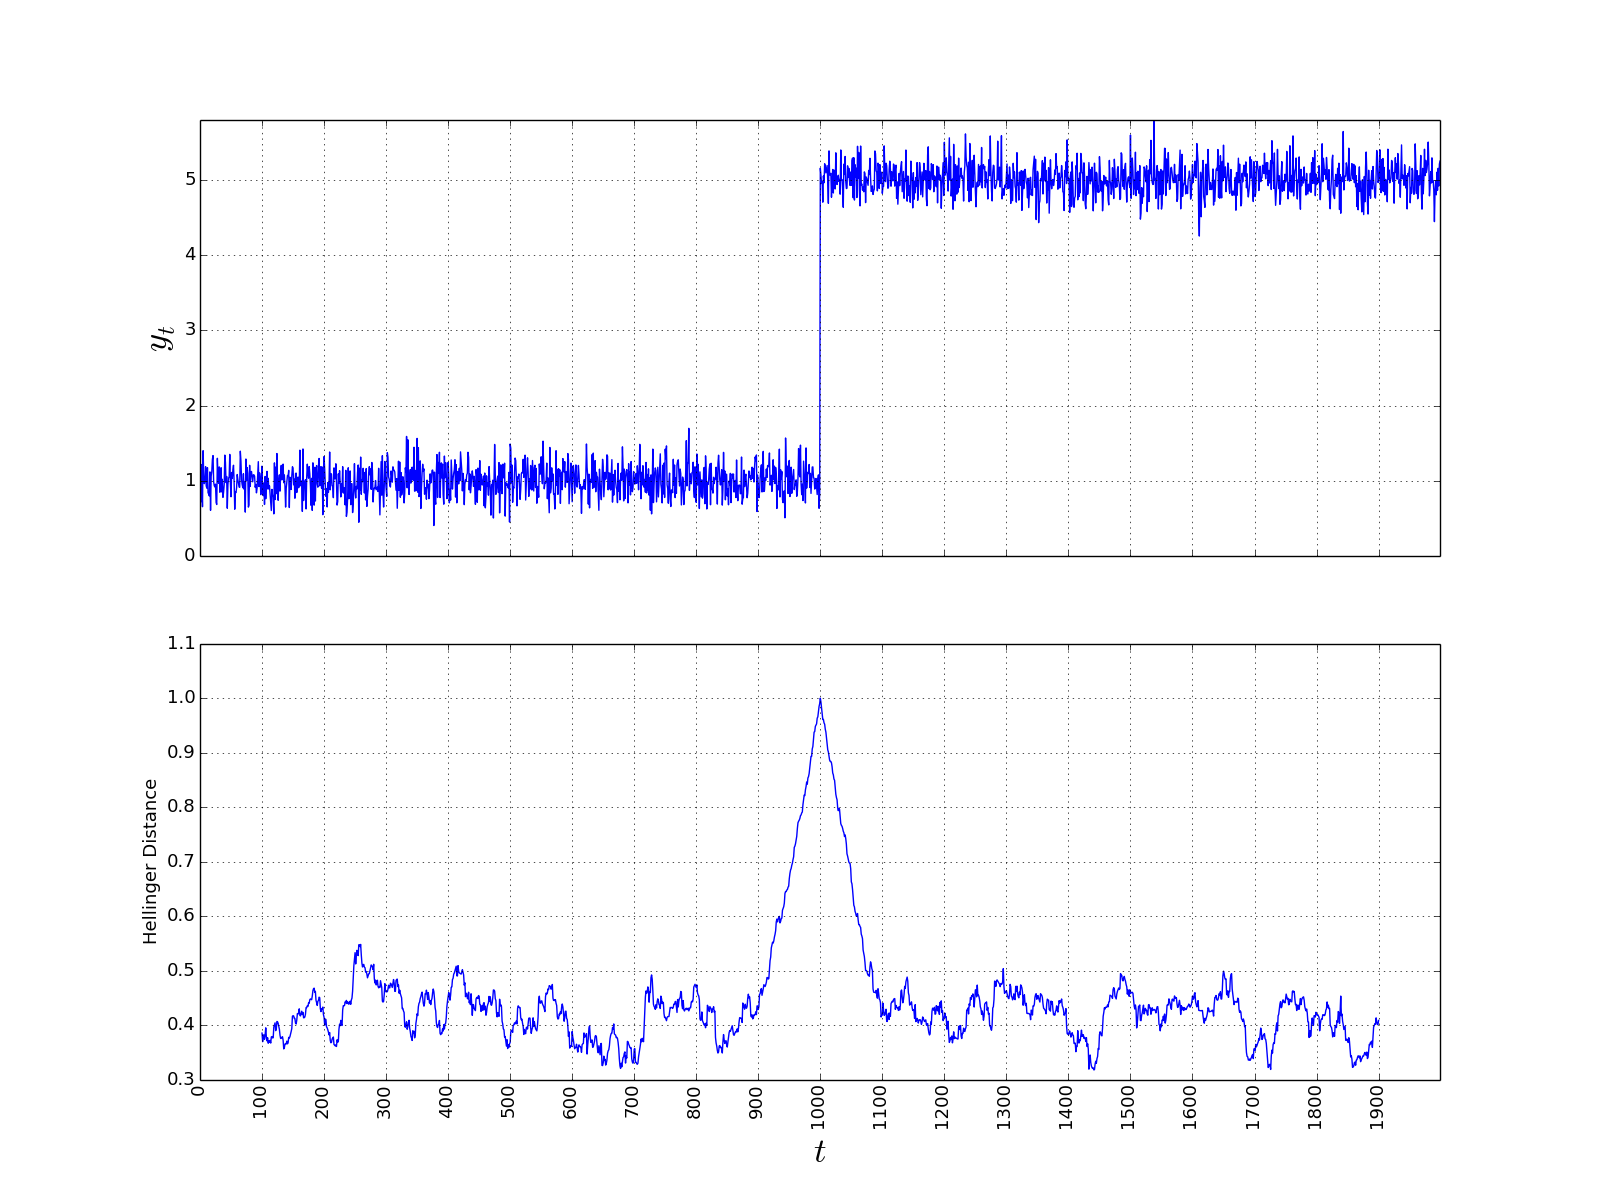
\includegraphics[width=1.0\textwidth]{./figures/sliding_window_toy_example.png}
    \caption{Toy example of sliding window.}
    \label{fig:sliding_window_toy_example}
\end{figure}

It can be observed that there is a peak on the distance in the exact location where the distribution changed. However, using only the threshold method is possible to prematuraly infer the location of the change point. Therefore, an alternative is to also use a peak detection algorithm in the distance of two sliding windows time series.

The distance function choice can significantly impact the performance. There are several empirical distribution distances such as mahalanobis distance, hellinger distance, jensen shannon and EMD (Earth Mover's Distance).  

A performance improvement can be achieved concurrently executing the same sliding window algorithm with different window lengths, which enable the segmentation with different windows sizes more easily.

\section{Optimization Model}  

Given a fixed value of $k$, one approach is to define a cost function that measure the homogeneity of a segment and therefore choose the change points that globally optimize this homogeneity. Let the cost of the $i$-th segment be defined as $C(\mathbf{y}_{\tau_{i - 1} + 1 : \tau_{i}})$. The cost of a segmentation is then the sum of all segments costs.

A commom choice for function $C$ is the MSE (Mean Squared Error) which can capture changes in the mean. Another usual approach is to consider distribution changes through negative maximum log-likelihood functions, considering that data within a segment is iid. 

Therefore, given a fixed $k$, the optimal segmentation is obtained through the following optimization problem, which is called the constrained case: 

\begin{equation}
    \min_{\boldsymbol \tau_{1 : k}} \sum \limits_{i = 1}^{k + 1} C(\mathbf{y}_{\tau_{i - 1} + 1 : \tau_{i}})
\end{equation}

This problem can be solved using dynamic programming with $O(k n^2 f(n))$ time complexity, where $f(n)$ is related with $C$ evaluation. Several segment cost functions can be evaluated in $O(1)$ after a $O(n)$ preprocessing phase, implying in an overall $O(k n^2)$ complexity. It is possible to proof that MSE, negative maximum log-likelihood function of normal, exponential, poisson and binomial distributions have this characterestic. Also the formulation can consider a minimum value of a segment length.

Modelling segments with continuous distributions can lead to practical dificulties. One of them is the fact that segments can form degenerate distributions, that is, the points of a segment can have zero variance, which is always the case of unitary length segments. In these cases the negative maximum likelihood are undefined. Two approaches can be used to avoid this situation. The first one tries to avoid degenerate segments adding a white noise with small variance to the time series. The second one considers that the cost of any degenerate distribution segment is equal to a small constant.

% Using discrete distributions it is possible to easily compare direct compare the likelihood of two different distribution types. 

% Since the likelihood of different continuous distributions can`t be directly compared, is not possible to apply the segmentation algorithm considering different types of continuos distributions. One possibility to handle this is to apply automatic methods to check which kind of distribution fits better to the segment, such as Kolmogorov-Smirnov. This was not approached in this work due to the computation time efficiency decrease and that since we deal with small number of data possibly these methods would have a poor performance.

When the number of change points is unknown a common approach is to introduce a non decreasing penalty function $g(k)$. Then the new optimization problem, called penalized case, is:

\begin{equation}
    \min_{k, \boldsymbol \tau_{1 : k}} \sum \limits_{i = 1}^{k + 1} C(\mathbf{y}_{\tau_{i - 1} + 1 : \tau_{i}}) + g(k)
\end{equation}

An approach to solve this problem is to solve the constrained case for $k = 0, ..., K$. This lead to an $O(K^{2} n^{2} f(n))$. However if the penalty function is linear in $k$ the problem can be formulated in a more efficiently and solved in $O(n^{2} f(n))$ time complexity with dynamic programming.

Also there are several pruning algorithms to speedup the computation, in general trying to reduce the $\boldsymbol \tau$ search space but maintaning optimality.

\section{HMM (Hidden Markov Model)}

The idea that each segment of the time series is associated with a specific latent parameter of the procedure that generated the time series has a direct interpretation to a HMM model. In this context, each segment of a time series is related to a hidden state of a HMM model, and the observation distribution of this state represents the distribution of that segment. Therefore, the mechanism is resumed to model the target time series using a HMM and assessing when occurs a transition between different hidden states in the hidden state path.

There are several approaches in the detection and training phase. For example, given a trained HMM is possible to analyze the most probable hidden state path that a time series can follow through the viterbi algorithm. Also is possible to evaluate the probability of a transition between different hidden states at time $t$ and apply a threshold method together with peak detection as in the sliding window method. For the training phase is possible to use several time series to train a single HMM and use this model to detect change points in all time series. Another way is to train a model using only a single time series to be processed.

It is important to note that structure of the hidden state graph has a big impact in the performance. Using a full connected structure the number of states defines the number of different distribution parameters of the different segments. Using a left to right structure the number of hidden states will induce the number of segments.

In \ref{} is stated that when using a full connected structure the time that a time series stays in the same hidden state is low, which can not reflect that fact that in real data the number of change points is also low. To overcome this problem \ref{} suggest to increase the time that a time series stay in the same hidden state through a dirichlet prior penalization.

\section{Bayesian Inference}

There are several bayesian methods for the change point detection problem. The work of \ref{} derive recursions based on a set of priors to assess the probability that a point is a change point in an offline fashion. The algorithm recursevely calculates, for each $i$, the probability of $\mathbf{y}_{i : n}$ given a change point at $i$. With these probabilities is possible to simulate the time of the first change point, and then, compute the conditional distribution of the time of the second change point given given the first, and so on. To achive this, the mechanism assumes that observations are independents, and that each segment is modelled by conjugate priors. Also, the model considers priors to model the number of change points and the time between two consecutive change points. The overall complexity of this method is O().




